	\documentclass[12pt]{article}
\usepackage{geometry}                
\geometry{letterpaper}               
\usepackage[parfill]{parskip}    	
\usepackage{graphicx}				
\usepackage{amsmath}
\usepackage{amssymb}
\usepackage{hyperref}
\usepackage{authblk}
\usepackage{xcolor}
\usepackage{xspace}

\title{Forecasting Model for the Spread of SARS-CoV-2}
\author{\sc David Champredon}
\affil{Department of Pathology and Laboratory Medicine \\Western University (London, Ontario)\\ \texttt{\small{david.champredon@gmail.com}}}
%\date{}							% Activate to display a given date or no date


\newcommand{\Ro}{\mathcal{R}_0}
\newcommand{\pois}{\mathrm{Poisson}}
\newcommand{\gam}{\mathrm{Gamma}}
\newcommand{\warning}[1]{\textbf{\textcolor{red}{#1}}\xspace}


\begin{document}
\maketitle


\warning{ Warning: This is a draft documentation and not as clear as I would like it to be: do not hesitate to contact me for any questions or comments. The model described here is a constantly evolving work and is used to provide daily forecasts to Public Health Ontario. A link to a Github repo will be posted soon.}

\section{Data}

The data used to fit the model are the confirmed (positive) COVID-19 cases that are considered a proxy for the true (unobserved) incidence of infections in the whole population. 
Moreover, to inform the generation interval distribution, I use data from line lists of COVID-19.
My data source for COVID-19 reports in Canada is compiled and curated by Michael Li (\href{https://github.com/wzmli/COVID19-Canada}{https://github.com/wzmli/COVID19-Canada}).


\section{Model}

\subsection{Reported cases and true incidence}
The number of positive cases reported at time $t$ is $P_t$ and the true, unobserved, incidence of infections is $I_t$. 
I assume a stochastic relationship between the positive reports and the true incidence:

\begin{equation}
I_t \sim \gam\left( \mathrm{mean}=\frac{P_{t+\ell}}{\rho} , \mathrm{cv}=v_{obs} \right)
\end{equation}

The probabilistic distribution is a convenient way to represent reporting errors and changes in the testing strategy. The shape parameter of this Gamma distribution is set such that the coefficient of variation $v_{obs}$ has a pre-determined value.
The parameter $\ell$ is a constant that represents the reporting delay. 

\subsection{Severity cascade}

I assume the numbers of hospitalized cases at time $H_t$ is directly proportional to the number of positive cases $P_t$. Similarly, the number of patients needing critical care (in ICUs with or without ventilators) $C_t$ is proportional to the hospitalized cases, and finally the number of deaths $D_t$ is proportional to the number of critically ill patients. Assuming again a stochastic relationship:

\begin{eqnarray}
H_t & \sim \pois(h\, P_t)\\
C_t & \sim \pois(k\, H_t)\\
D_t & \sim \pois(d\, C_t\, e^{\varepsilon t})
\end{eqnarray}

The term $e^{\varepsilon t}$ is an adjustment for the different growth rate observed between death and reported cases. The parameter $\varepsilon$ is fitted on data. 


\begin{figure}[htbp]
\begin{center}
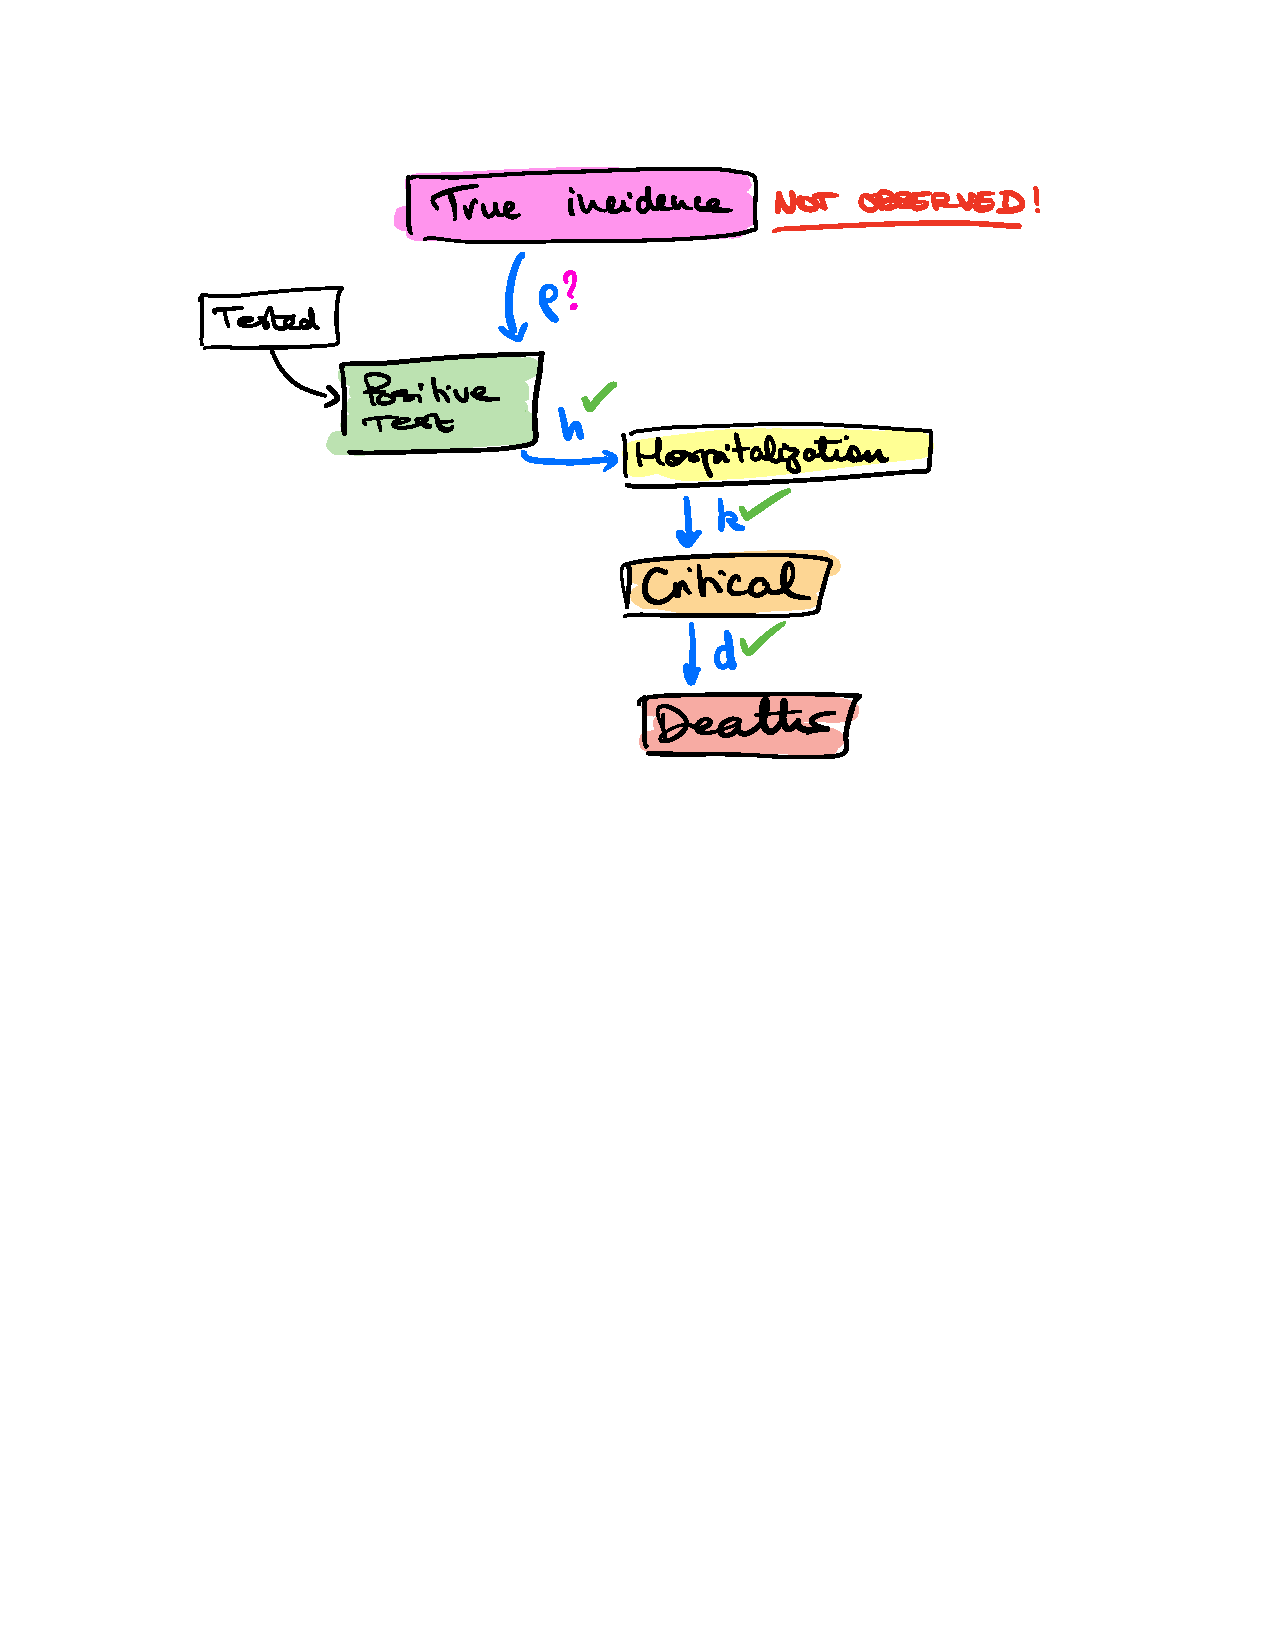
\includegraphics[width = 0.6\textwidth]{cascade.pdf}
\caption{Model of the severity cascade of COVID-19 cases}
\label{fig:cascade}
\end{center}
\end{figure}




\subsection{Transmission process}

I use a probabilistic representation of the renewal equation to model the disease transmission process:

\begin{equation}
I_t  \sim \gam (m_t , \phi) \\
\end{equation}

with $\phi$ a dispersion parameter and $m$ the mean incidence defined as 

\begin{equation}
m_t  =  \left( \frac{S_t}{N}  \right)^{1+\alpha} \Ro \, B_t \sum_{j\geq 1} I_{t-j}g(j)
\label{eq:renewal}
\end{equation}


where $g$ is the intrinsic generation interval distribution; $\alpha$ is a parameter modelling the mixing heterogeneity ($\alpha=0$ means homogeneous mixing; the larger $\alpha$, the more heterogeneous the implicit contact structure); $N$ is the effective population size; $\Ro$ the basic reproduction number; and $B_t$ a function  that models behavioural change at time $t$.

The function $B_t$ can take various shapes in order to represent different intervention scenarios. 
\begin{figure}[htbp]
\begin{center}
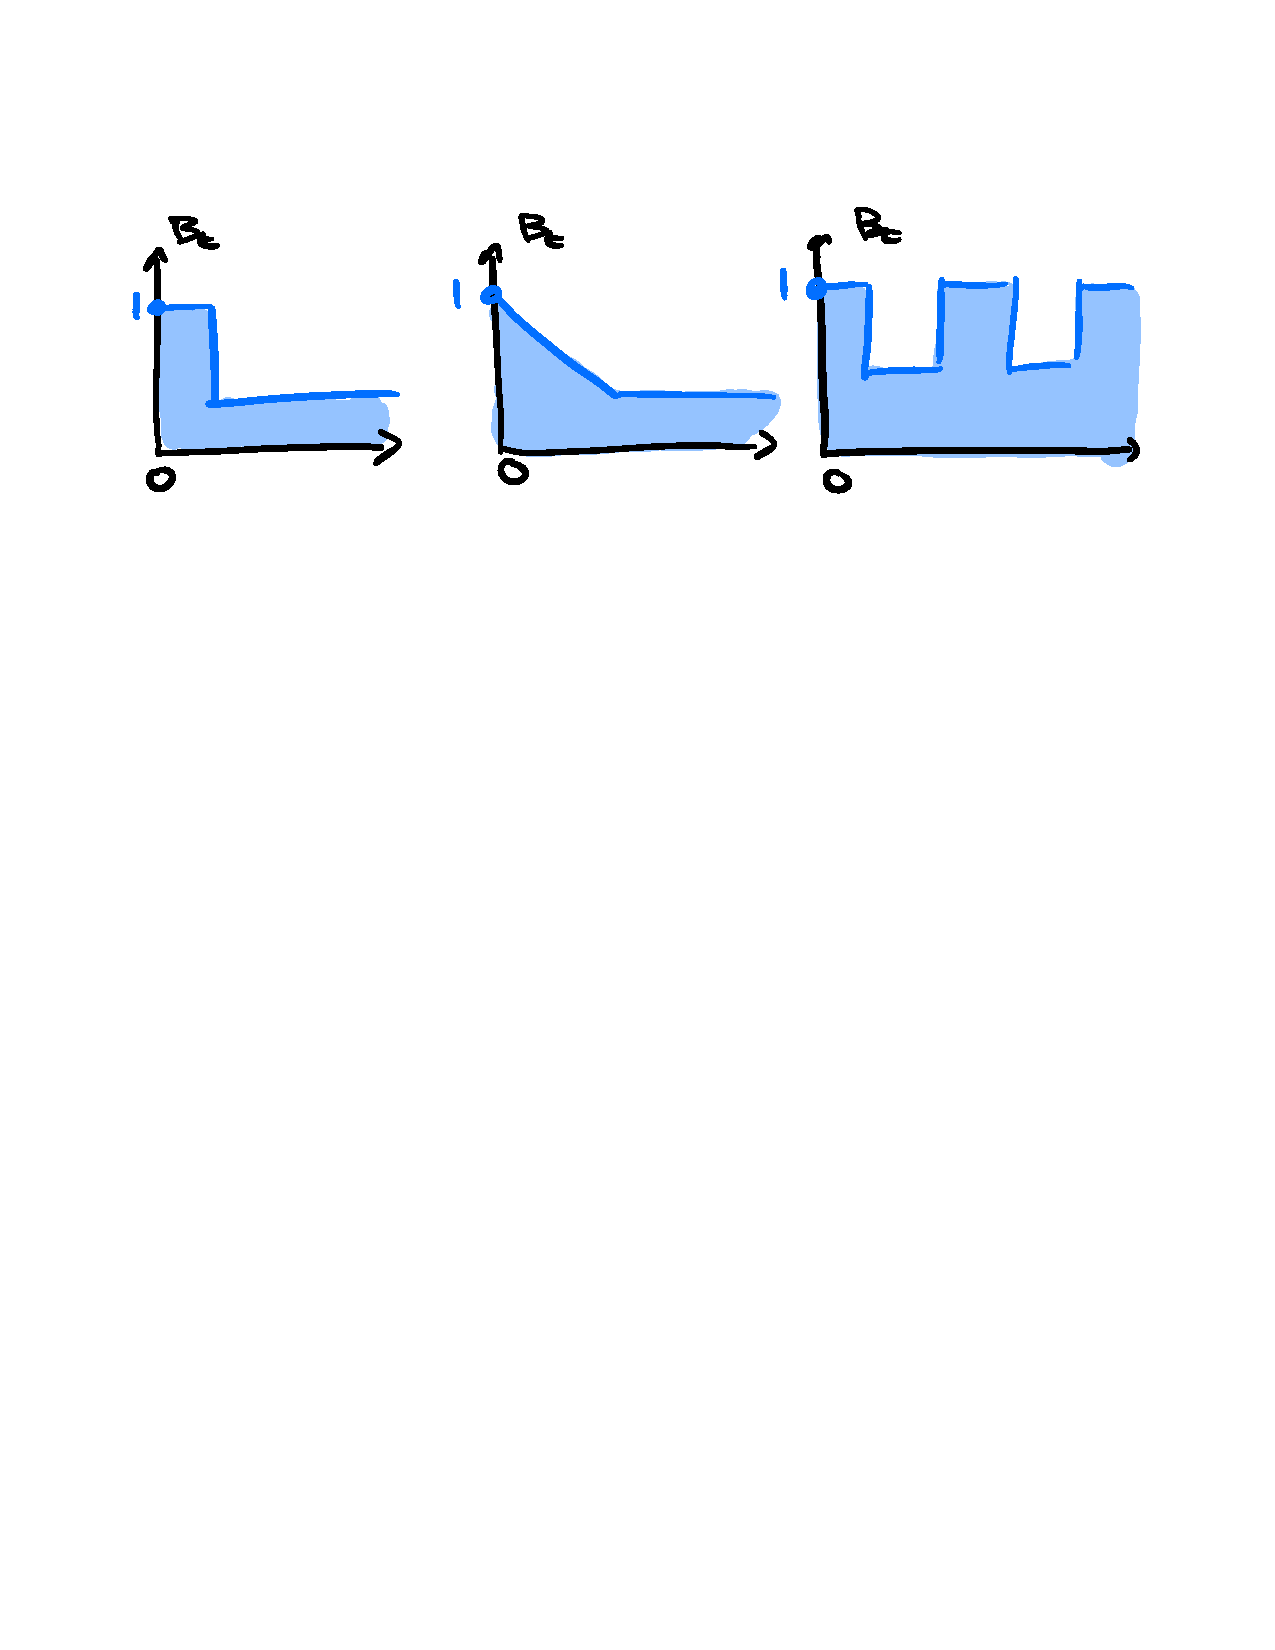
\includegraphics[width = 0.8\textwidth]{Bt.pdf}
\caption{Examples of possible shape for $B_t$ to represent interventions.}
\label{fig:Bt}
\end{center}
\end{figure}



\section{Fitting}

\subsection{Exponential growth phase}

The generation interval is informed by available line lists of COVID-19 cases worlwide. 

The basic reproduction number $\Ro$ is fitted on the positive tests reported using the Dushoff and Park Gamma moment approximation:
\begin{equation}
\Ro = (1 + \kappa r \bar g) ^{1/\kappa}
\label{eq:approxGammaR0}
\end{equation}
where $r$ is the exponential growth rate of positive cases reported, $\bar  g$ is the mean generation interval and $\kappa$ a dispersion parameter informed by the observed variance of the generation interval.

The growth rate $r$ is estimated with a linear regression on the log number of positive tests. The confidence interval are used to propagate uncertainty in $\Ro$ and consequently in the transmission process via the renewal equation \autoref{eq:renewal}


The parameters for the severity cascade are directly observed from the daily epidemiological reports.

\subsection{Deceleration phase}

When the incidence count start to deviates from an exponential growth, the approximation defined by \autoref{eq:approxGammaR0} is not valid anymore. 

In this ``deceleration'' phase, the model parameters are fitted using an approximate bayesian computation method (ABC). More specifically, the parameters $\Ro$, $\alpha$ and potentially $B_t$ are fitted jointly on the incidence curve. 
For example, to assess the effect of social distancing in Ontario, I take $B_t$ as a Heaviside step function with a discontinuity at the time of the declaration of the state of emergency (March 17, 2020) and a step size of $1-\lambda$ (so $\lambda$ is the effect of the intervention).

The distribution prior used are listed in \autoref{tab:priors}.

\begin{table}[h!]
\caption{}
\begin{center}
\begin{tabular}{cc p{6cm}}
\hline
\bf Parameter & \bf Prior & \bf Comments \\
\hline
$\Ro$ & Normal(2, 0.7) & weak prior\\
$\alpha$ & Uniform(3, 5) & strong prior: contact structure highly heterogeneous\\
$\lambda$ & Uniform(0, 1) & weak prior \\
\hline
\end{tabular}
\end{center}
\label{tab:priors}
\end{table}%

The fit on Ontario data shows that $\Ro$ and $\lambda$ are well identified by a unimodal posterior distribution but the posterior distribution of the heterogeneity parameter $\alpha$ is, unsurprisingly, not informed by the data.


\section{Model Parameters}



\renewcommand{\arraystretch}{1.3} 
\begin{table}[h!]
\begin{center}
\begin{small}
\begin{tabular}{l c p{6cm}}
\hline
\bf Parameter & \bf Value & \bf Comments \\
\hline
Basic reprod. num. $\Ro$ & fitted  & \autoref{eq:approxGammaR0} or ABC\\
Contact heterogeneity $\alpha$ & fitted & arbitrary strong prior\\
Intervention effect $\lambda$ & fitted & weak prior \\
Mean generation interval & 4.5 days & from various studies \\
Variance of generation interval & 7 days$^2$ & from various studies \\
Susceptible proportion &  0.8  & assumption \\
Prop. of true incidence reported positive & Beta(20, 60) & CMMID \\
Prop. of positive to hospitalized $h$ & 0.14 & Daily report from PHO; adj. daily\\
Prop. of hospitalized to critical $k$ & 0.39 & Daily report from PHO; adj. daily \\
Prop. of critical to death $d$ & 0.60 & Daily report from PHO; adj. daily \\
Coeff. of variation obs. process $v_{obs}$ & 0.2 & assumption\\
Dispersion of transmission process $\phi$ & 0.7 & assumption\\
\hline
\end{tabular}
\end{small}
\end{center}
\label{tab:parameters}
\end{table}%




\end{document}  




